\documentclass{beamer}
\usetheme{LHC}
\usepackage[utf8]{inputenc}
\usepackage[T1]{fontenc}
\usepackage{hyperref}

%% Use any fonts you like.
\usepackage{helvet}

\title{Summer Student Project}
\subtitle{An alternative approach to configure permanent tasks in LHCb Online farm nodes}
\author{Krzysztof Wilczyński}
\date{August 28, 2018}
\institute{Supervisors: Markus Frank, Beat Jost}

\begin{document}

\begin{frame}[plain,t]
\titlepage
\end{frame}


\section{Introduction}
\begin{frame}
\frametitle{About me}
\subsection{About me}

\begin{center}
\begin{itemize}
\item I am... an engineer!
	\begin{itemize}
	\item Master student of Automatic Control and Robotics\\ 			(spec. Robotics)
	\item Faculty of Power and Aeronautical Engineering, \\
    	Warsaw University of Technology
	\end{itemize}
\end{itemize}
\end{center}

\noindent\begin{minipage}{0.5\textwidth}
%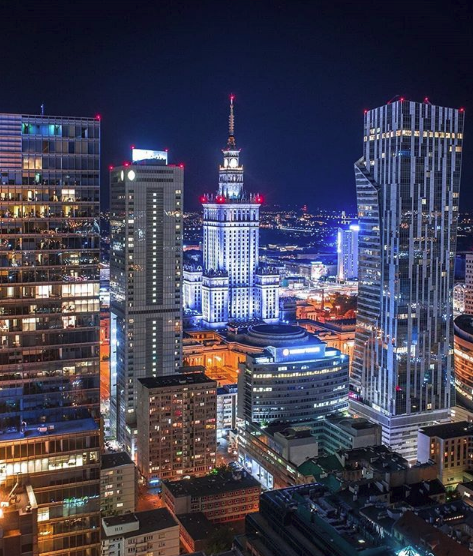
\includegraphics[width=\linewidth]{warsaw1}
\begin{itemize}
\item I used to work at...
	\begin{itemize}
	\item Bosch Rexroth
	\item Airbus Military Defence and Space
    \item Student Association for Vehicle Aerodynamics
    \item Polish National Opera
	\end{itemize}
\end{itemize}
\end{minipage}%
\hfill%
\begin{minipage}{0.5\textwidth}\raggedleft
\begin{figure}
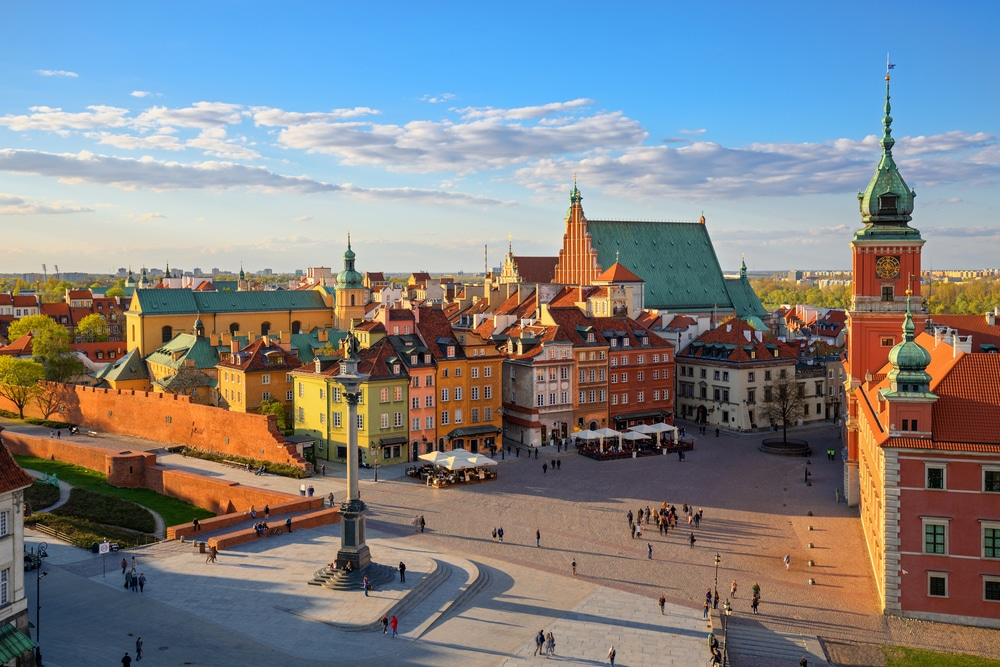
\includegraphics[scale=0.13]{images/warsaw2}
\end{figure}
\end{minipage}


\end{frame}

\section{The system}

\begin{frame}
\frametitle{Online farm computing nodes}
\subsection{Online Farm}
\begin{figure}[H]
    	\centering
    	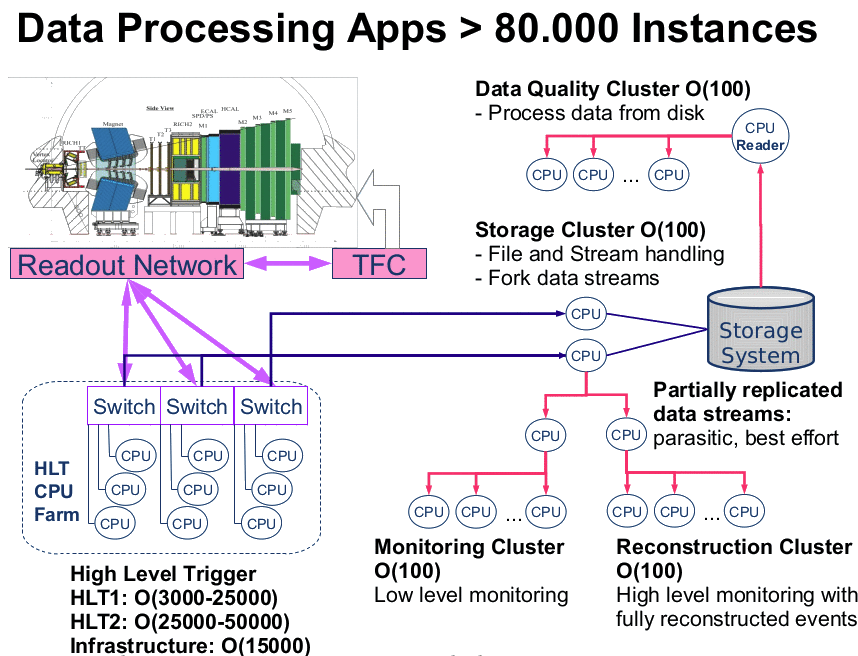
\includegraphics[scale=0.3]{images/Farm.png}
\end{figure}
\end{frame}



\subsection{Farm controller}
\begin{frame}
\frametitle{LHCb Online farm process controller}

The handling of the permanent processes on the data processing nodes is based on sending commands to pcSrv process running on each of the corresponding "Controls PCs".
\newline


\underline{
\href{https://www.researchgate.net/publication/268357086_The_Process_Controller_for_the_LHCb_On-Line_Farm_Prepared_by}{LHCb Online Farm Process Controler on Researchgate}}
% \hyperref[Documentation]{""}

\end{frame}

\subsection{Boot script}
\begin{frame}
\frametitle{Farm boot script}

\noindent\begin{minipage}{0.6\textwidth}
In the current solution, all processes (scripts) started on the farm nodes are grouped in a single, huge python script that prints out ready to execute pcAdd commands for a given node name.
\end{minipage}%
\hfill%
\begin{minipage}{0.4\textwidth}\raggedleft
\begin{figure}

\includegraphics[scale=0.5]{images/on.jpeg}
\end{figure}
\end{minipage}
\vfill

\begin{block}{A command used to start a task on node(s):}
pcAdd(regex, start parameters, script, script parameters)
\end{block}

\end{frame}

\begin{frame}
\frametitle{Farm boot script}

\begin{itemize}
\item The main disadvantages of the solution:
\begin{itemize}
\item Modifications of task parameters are difficult
\item It is easy to make a modification that harms dependencies in the task sets (no error prevention mechanism)
\item Only a specialist who knows the boot script structure can use it (no high-level interface)
\item There is no easy way of knowing which tasks are running on given node (one has to analyze the boot script line by line)
\end{itemize}
\end{itemize}
\vfill
\begin{block}{The boot script has been created as a "quick hack" about 10 years ago. \\ The time has come to upgrade it!}
\end{block}
\end{frame}




\section{The motivation}
\begin{frame}
\frametitle{My project}
\subsection{Upgrades}
\begin{block}{The solution: create a system for the process controller infrastructure utilizing a database driven approach. The main goals were to:}
\begin{itemize}
\item simplify the modifications of hierarchical structure of tasks running on the nodes
\item prevent human errors breaking the system integrity
\item create one source of information regarding processes running on a given node
\item create a reliable and future-proof API for future developments
\end{itemize}
\end{block}
\end{frame}

% In short, the above goals can be achieved using a cleverly designed system using database approach rather than a "hardcoded" parameters boot script. 

\begin{frame}
\subsection{API}
\frametitle{What do I mean by Main API?}
\begin{figure}[H]
	\centering
    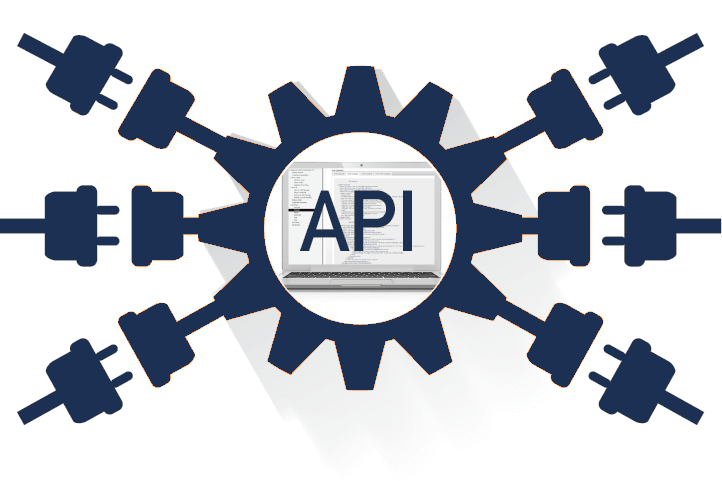
\includegraphics[scale=0.22]{images/api.png}
\end{figure}
\begin{block}{API: Application Programming Interface}
The created API is a Python class containing methods (add, delete, modify, get, assign, inSet) that allow safe access to the underlying database. It is a high-level connector providing an easy integration of different client applications.
\end{block}

\end{frame}


\begin{frame}
\frametitle{Stages of development}
\subsection{Development}

\begin{block}{Back-end}
\begin{itemize}
\item Database schema architecture
\item Main database API
\item New boot script
\item Unit testing script (internal error prevention)
\item Frontend connectors: JSONRPC, (REST, XMLRPC)
\end{itemize}
\end{block}
\begin{block}{Front-end}
\begin{itemize}
\item Command line user interface
\item Graphical user interface (web application)
\end{itemize}
\end{block}

\end{frame}

\section{The results}
\begin{frame}
\frametitle{Current results}
\subsection{Results}
\begin{figure}[H]
    	\centering
    	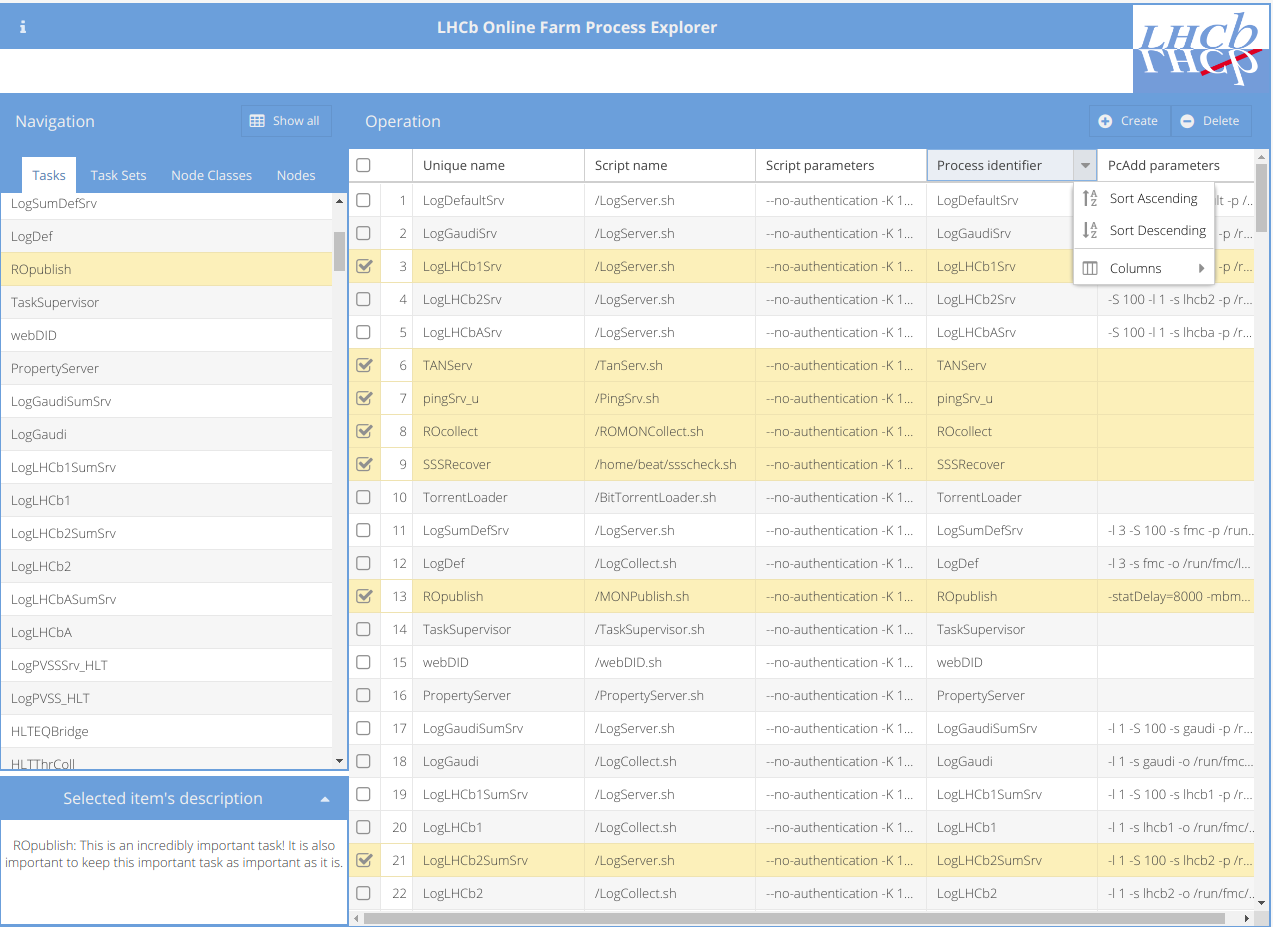
\includegraphics[scale=0.15]{images/gui.png}
\end{figure}
%\begin{block}{Live demonstration!}
%\end{block}
\begin{block}{Open-source code repositories:}
\begin{itemize}
\item \underline{\href{https://bitbucket.org/3sztof/lhcb_online/src/master/}{Bitbucket Repository (K. Wilczynski)}} 
\item Will be moved to LHCb Gitlab Repository (M. Frank)
\end{itemize}
\end{block}
\end{frame}

\begin{frame}
\frametitle{Tools used in the project}
\subsection{Tools}

\begin{itemize}
\item Back-end programming language: Python 2.7.15rc1
\item Front-end programming language: JavaScript
\item Database engine: SQLite (+ python sqlite3, sqlalchemy)
\item Front-end connector protocol: JSONRPC
\item Front-end framework: Sencha Ext JS ver. 6.2.0
\item Git version control: Bitbucket + GitKraken
\end{itemize}

\end{frame}

\ThankYouFrame

\begin{frame}
\frametitle{Task grouping hierarchy}
\begin{figure}[H]
    	\centering
    	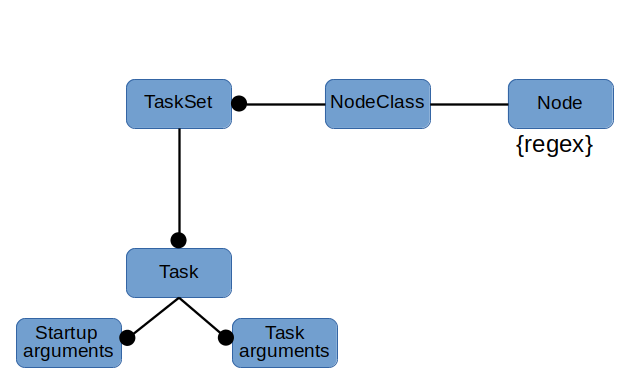
\includegraphics[scale=0.4]{images/hierarchy.png}
\end{figure}
\end{frame}

% \subsection{Blocks}
% \begin{frame}
% \frametitle{Blocks}
% \begin{definition}[Greetings]
% Hello World
% \end{definition}

% \begin{theorem}[Fermat's Last Theorem]
% $a^n + b^n = c^n, n \leq 2$
% \end{theorem}

% \begin{alertblock}{Uh-oh.}
% By the pricking of my thumbs.
% \end{alertblock}

% \begin{exampleblock}{Uh-oh.}
% Something evil this way comes.
% \end{exampleblock}

% \end{frame}

\end{document}